\chapter*{Inner Simulator}


\section*{Epistemic status: Firm}
\setlength{\parindent}{0em}
\begin{spacing}{.85}
\emph{\small{The concepts underlying the Inner Simulator model (and the related practical technique of Murphyjitsu) are well-known and well-researched, including Kahneman's S1/S2, mental simulation, and mental contrasting.  Similarly, the problems that this unit seeks to address (such as optimism bias and the planning fallacy) have been studied in detail.  There is some academic support for specific substeps of Murphyjitsu (e.g. prospective hindsight), and strong anecdotal support (but no formal researc) for the overall technique, which was developed through iterated experimentation and critical feedback.  See the Further Resources section for more discussion.}}
\end{spacing}

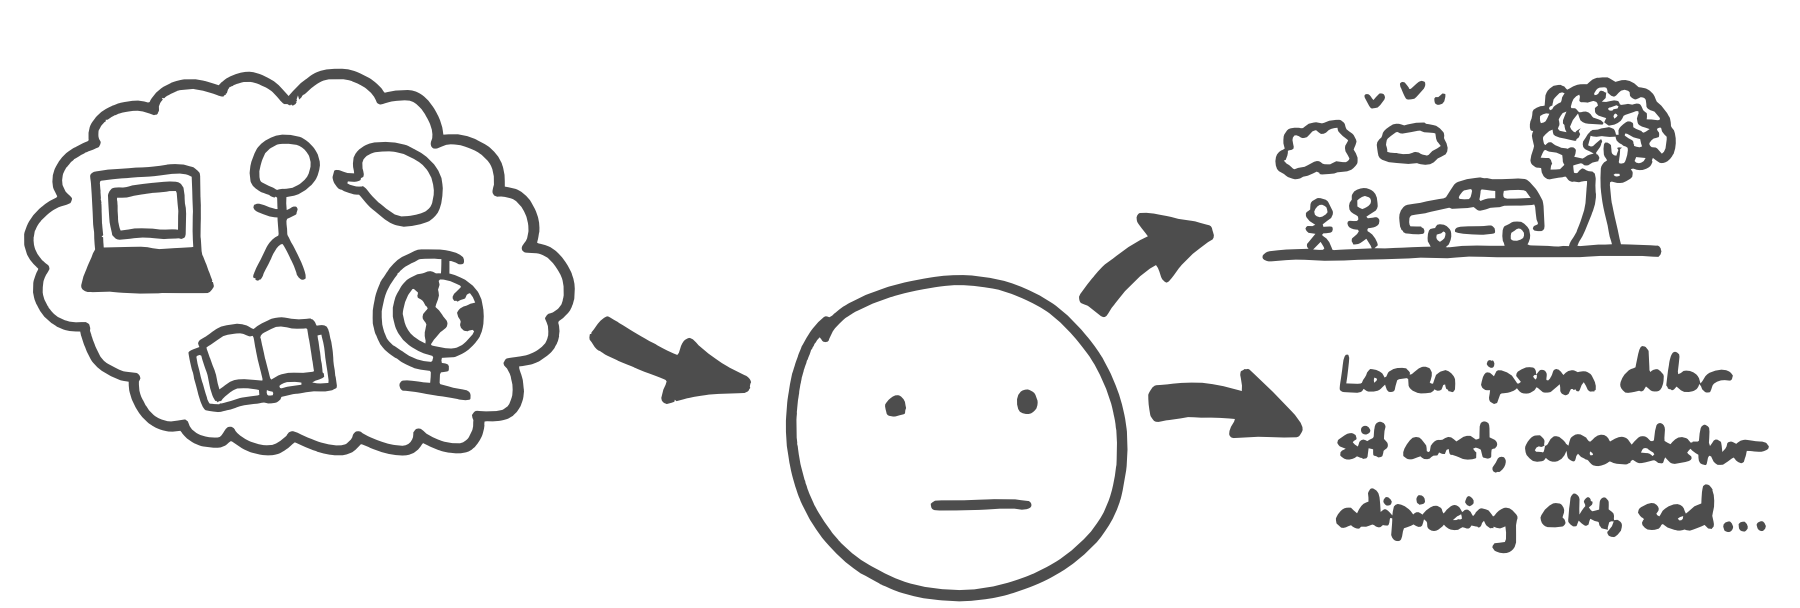
\includegraphics[width=\textwidth]{../../../img/innersim01.png}
\setlength{\parindent}{1.5em}

When you move to catch a falling pen, or notice that your friend is upset just by the way they entered the room, you're using your \textbf{inner simulator}.  It's a different sort of processing from the explicit/verbal stuff we usually call ``thinking,'' and it results in a very different kind of output.
\\
\begin{table}[h] \small \centering
	\begin{tabular}{ | p{.45\textwidth} | p{.45\textwidth} | }
		\hline
		\textbf{Inner Simulator} & \textbf{Explicit/Verbal Models} \\ \hline
		Intuitive; part of System 1 & Analytical; part of System 2 \\ \hline
		Outputs feelings, urges, reflexes, and vivid predictions & Outputs arguments, calculations, and explicit models \\ \hline
		Learns well from experience and examples; responds to being \emph{shown} & Learns well from facts and explanations; responds to being \emph{told} \\ \hline
		Good at social judgment, routine tasks, and any situation where you have lots of experience & Good at comparisons and reframings (e.g. noticing that \$1/day $\approx$ \$350/year) \\ \hline
	 \end{tabular}
\end{table}
\medskip

Each of us carries around a rich, complex model of the universe in our head, assembled from a lifetime of experiences and memories.  We don't have to \emph{think} about how to catch a falling pen, because our inner simulator \emph{knows} how falling objects move.  Similarly, it knows what facial expressions mean, what it's like to drive from home to work, and what sorts of things \emph{tend to go wrong} given a set of circumstances.  It's a powerful tool, and learning how to access it and when to trust it is one of the first steps to becoming a whole-brain thinker.

That's not to say that your inner simulator is \emph{superior} to your explicit model maker---each has both strengths and weaknesses, and can be either the right tool or the wrong one, depending on the situation.  In any given moment, you're probably receiving feedback from both of these ``advisors,'' as well as other sources of information like your friends or the internet.  

In a sense, it's your job to balance the competing recommendations from all of these different advisors to arrive at the best possible decision.  Your inner sim, for example, provides feedback extremely quickly and is good at any type of task where you have lots of experience to draw on, but tends to fall prey to framing effects and will sometimes sneakily substitute an easy question for a harder one.  Your explicit verbal models, on the other hand, are great for abstractions and comparisons (such as noticing that \$1/day $\approx$ \$350/year), but are slow and vulnerable to wishful thinking and ideological distortions.\footnote{In some situations, \emph{neither} of these advisors is sufficient.  Imagine someone who's never driven on ice before starting to skid---their inner sim will likely ``tell'' them to slam on the brakes before their explicit verbal models has time to offer up the sentence \emph{don't slam on the brakes when you're skidding on ice.}  Yet leaving those slooooooooow verbal models in control of the driving process is a terrible idea in its own right, like trying to catch a ball by first explicitly calculating its trajectory according to physics equations.}

You can think of your inner sim as a black box that's capable of performing a few specific functions, given certain input.  It's very, very good at doing those functions, and not so great with most other things (for instance, inner sim is terrible at understanding large numbers, and causes us to donate \emph{the same amount of money} to save 8,000 or 800,000 hypothetical birds from oil spills).  But if you need a particular kind of reality check, it helps to know which parts of reality inner sim sees most clearly.

\setlength{\parindent}{0em}
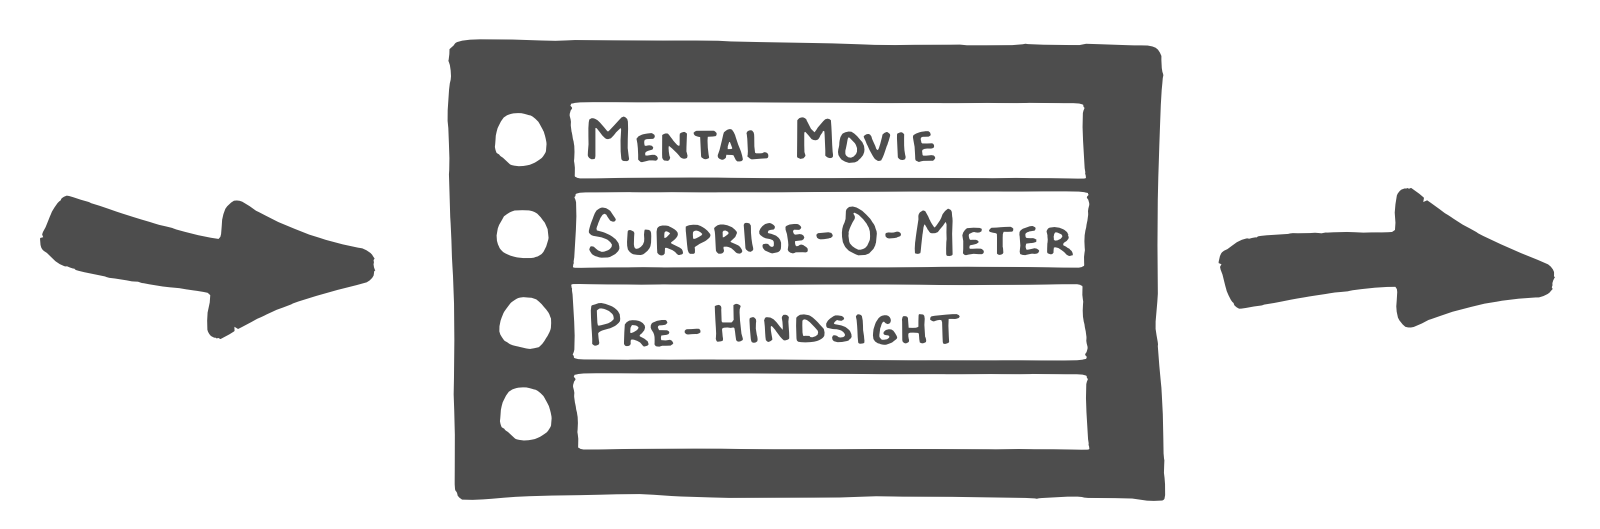
\includegraphics[width=\textwidth]{../../../img/innersim02.png}
\setlength{\parindent}{1.5em}

\section*{Prompts for your inner sim}

\subsubsection{What happens next?}
Start a ``mental movie'' by concretely visualizing a situation, and see what your brain \emph{expects to happen.}  If this is the beginning of the scene, how does the scene end?
\begin{itemize}
	\item \textbf{Input:} A laptop is balanced on the edge of a table in a busy office.
	\item \textbf{Input:} You lift a piece of watermelon to your mouth and take a bite.
	\item \textbf{Input:} You sneak up on your closest colleague at work, take aim with a water gun, and fire.
\end{itemize}

\subsubsection{How shocked am I?}
Check your ``surprise-o-meter''---visualize a scenario from start to finish, and see whether you ``buy'' that things would actually play out that way.  Common outputs are ``seems right/shrug,'' ``surprised,'' and ``shocked.''
\begin{itemize}
	\item \textbf{Input:} You've purchased food to feed twenty-five people at your party, and only ten people show up.
	\item \textbf{Input:} Same party, but \emph{seventy} people show up.
	\item \textbf{Input:} You finish your current project in less than half the time you allotted for it.
\end{itemize}

\subsubsection{What went right/wrong?}
Use your ``pre-hindsight''---start by assuming that your current plan has utterly failed (or gone perfectly, but that's the side we're already biased toward believing).  What explanation leaps to mind about why this happened?
\begin{itemize}
	\item \textbf{Input:} Think of a \emph{specific} email you intend to send next week.  Turns out, the person you sent it to was extremely irritated by it.
	\item \textbf{Input:} Imagine you receive a message from yourself from the future, telling you that you should \emph{absolutely} stay at your current job, and keep up the good work.
	\item \textbf{Input:} It's now been three months since your CFAR workshop, and you have yet to make deliberate use of your inner simulator.
\end{itemize}

\section*{Making good use of your inner simulator}
Like most algorithms, your inner simulator will output good and useful information if you give it good and useful input, and it will output useless garbage if that's what you feed it.  It's an especially good check on wishful thinking and motivated cognition---just imagine its response to a list of New Year's resolutions---but you need to make sure that you aren't rigging the game by phrasing questions the wrong way.

Two useful strategies for avoiding vague, open-ended ``garbage'' are sticking to \emph{concrete examples} and looking for \emph{next actions}.

\subsubsection{Asking for Examples}
\newenvironment{blockquote}{\par \medskip \leftskip=1.5em \rightskip=1.5em \noindent\ignorespaces}{\par\medskip}
\begin{blockquote}
``It's just so \emph{frustrating.}  It's like, every little thing turns into a fight, you know?  And then it's \emph{my} fault that we're fighting, and I have to either pick between defending myself or smoothing things over, and since I'm the only one who ever wants to smooth things over, that means that I'm always the one apologizing.  And last week---I told you about what happened while we were stuck in traffic, right?  No?  So, like, out of \emph{nowhere,} while I'm trying to focus on not getting into a wreck, all of a sudden we're back talking about grad school \emph{again}\ldots''
\end{blockquote}

In a situation like this, your inner sim has nothing to grab onto---everything is vague, everything is open to interpretation, and clich\'es and stereotypes are filling in for actual understanding.  It could be that your friend is in the right, and needs your commiseration; it could be that the situation calls for some harsh truths and tough love.  How can you tell, one way or another?  Try some of these:
\begin{itemize}
	\item{What were the last couple of things you fought about?}
	\item{What were you talking about right before grad school came up?}
	\item{When you say you're the only one who wants to smooth things over, what do you mean?  What are you seeing and hearing that give you that sense?}
\end{itemize}

When it's just ``every little thing turns into a fight,'' your inner sim literally doesn't know what to think---there are too many possibilities.  But when the argument started with ``Do we really have to go over to Frank's \emph{again?}'' or with ``Oh, hey, I see you got new shoes.  Nice!'' you have a much better clearer sense of what the situation really looks like.

Asking for examples is a handy technique for any conversation.  When you keep your inner simulator engaged, and keep feeding it data, you might notice that it's easier to:

\begin{itemize}
	\item{\textbf{Notice when your friend's claim is false.}  In particular, if you keep your attention focused on concrete detail, you'll be more likely to notice \emph{where} the error is, instead of just having a vague sense of something ``not adding up.''}
	\item{\textbf{Notice if you're misunderstanding your friend.}  When we listen to someone else, we often try to approximate and anticipate what they're explaining.  If you keep asking for examples, you'll be more likely to notice if you've been accidentally adding or leaving out important features of the topic at hand.}
	\item{\textbf{Notice if \emph{you're} the one who's wrong.}  It's easy to avoid noticing if you've made a mistake---it's painful!  The more concrete your disagreement, the easier to notice if there's a flaw in your own argument, and to update accordingly.}
\end{itemize}

\subsubsection{Searching for Next Actions}
\begin{blockquote}
``I'm pretty excited about next year.  I'm going to finish paying off my loan, and once the weather gets better, I think I'm going to start running again.  Oh!  And I've been talking to some friends about maybe taking a trip to Europe---that is, if I don't end up going back to school.''
\end{blockquote}

A \emph{goal} isn't the same thing as a \emph{plan}.  I might have the goal of exercising more, but if I'm going to make that goal a reality---especially given that I'm not \emph{currently} exercising as much as I ``should''---then I'll need to think about when and how I'll get to the gym, what I'll do when I get there, what the realistic obstacles are going to be, and how I'm going to hold the plan together moment by moment and month by month.

But even before I get to those things, I'll need to take my \emph{next action}, which might be printing out a gym coupon, or setting a reminder in my calendar, or looking at my schedule for a good time to buy workout clothes.  A next action is a step that sets your plan in motion---it's both the first thing you'd have to do to build momentum, and also the first roadblock, if left undone.  Usually it's not particularly exciting or dramatic---next actions are often as mundane as putting something on the calendar or looking something up online.  If you're not able to take your next action at the moment you think of it, it's generally helpful to think of a \emph{trigger}---some specific event or time that will remind you to follow through.

For instance, if I have a \emph{goal} of applying to a particular school next fall, then my \emph{plan} will likely involve things like updating my CV, looking at the application process online, checking my finances, creating a list of plausible contacts for letters-of-recommendation, making decisions about work and relationships, and a host of other things.  If, after thinking it through, I decide that my \emph{next action} is to spend half an hour on the school's website, then I need a solid trigger to cause me to remember that at the end of a long day and a long commute, when I get home tired and hungry and Netflixy.  That trigger might be a phone alarm, or an email reminder in my inbox, or a specific connection to something in my evening routine---\emph{when I hear the squeak of my bedroom chair, I'll remember to go online}---but whatever trigger I choose, I'll be better off having one than not, and better off with a concrete, specific one than a vague, forgettable one.
\clearpage
\section*{Murphyjitsu: An Inner Sim Algorithm}
Murphy's Law states ``Anything that \emph{can} go wrong, \emph{will} go wrong.''  Even worse, people are notoriously bad at applying Murphy's Law when making plans and predictions---in a classic experiment, 37 psychology students were asked to estimate how long it would take them to finish their senior theses ``if everything went as poorly as it possibly could,'' and they \emph{still} underestimated the time it would take, as a group (the average prediction was 48.6 days, and the average actual completion time was 55.5 days).

However, where straightforward introspection fails, a deliberate use of inner sim can provide a valuable ``second opinion.''  Below are the steps for \textbf{Murphyjitsu}, a process for bulletproofing your strategies and plans.
\begin{itemize}
	\item{\textbf{Step 0: Select a goal.}  A habit you want to install, or a plan you'd like to execute, or a project you want to complete.}
	\item{\textbf{Step 1: Outline your plan.}  Be sure to list next actions, concrete steps, and specific deadlines or benchmarks.  It's important that you can actually visualize yourself moving through your plan, rather than having something vague like \emph{work out more}.}
	\item{\textbf{Step 2: Assume failure.}  It's been months, and you've made little or no progress!  Check your \textbf{surprise-o-meter}---where are you, on the scale from \emph{yeah, that sounds right} to \emph{I literally don't understand what happened}?  If you're completely shocked---good job, your inner sim endorses your plan!  If you're not, though, go to Step 3.}
		\item{\textbf{Step 3: Explain yourself.}  Using your \textbf{pre-hindsight}, try to construct a plausible narrative for what got in the way of success.\footnote{\textbf{Rampant speculation:} It seems plausible that the reason this works (where simply asking ``what could go wrong?'' fails) is that, in our evolutionary history, there was a strong selection pressure in favor of individuals with a robust \emph{excuse-generating mechanism}.  When you're standing in front of the chief, and he's looming over you with a stone ax and demanding that you explain yourself, you're much more likely to survive if your brain is good at constructing a believable narrative in which it's \emph{not your fault}.}}
		\item{\textbf{Step 4: Build in failsafes.}  What actions can you take to prevent these hypothetical failure modes?  Visualize taking those preemptive actions and then ask your inner sim ``What comes next?''  Have you successfully defused the danger?}
		\item{\textbf{Step 5: Iterate steps 2-4.}  That's right---it's not over yet!  Even with your new failsafes, your plan \emph{still failed.}  Are you shocked?  If so, victory!  If not---keep going.}
\end{itemize}

\section*{Inner Simulator---Further Resources}

\setlength{\parindent}{0em}
Kahneman and Tversky (1982) proposed that people often use a simulation heuristic to make judgments.  Mental simulation of a scenario is used to make predictions by imagining a situation and then running the simulation to see what happens next, and it is also to give explanations for events by mentally changing prior events and seeing if the outcomes changes.

Kahneman, D. \& Tversky, A. (1982). The simulation heuristic. In D. Kahneman, P. Slovic, \& A. Tversky (eds.) \emph{Judgment under uncertainty: Heuristics and biases} (pp. 201-208).

\hrulefill

Research on mental simulation has found that imagining future or hypothetical events draws on much of the same neural circuitry that is used in memory.  The ease with which a simulated scenario is generated often seems to be used as a cue to the likelihood of that scenario.  For a review, see:

Szpunar, K.K. (2010). Episodic future thought: An emerging concept. \emph{Perspectives on Psychological Science}, 5, 142-162.  http://goo.gl/g0NNI

\hrulefill

``Mental contrasting,'' sometimes referred to as \emph{gain-pain movies}, is a specific algorithm for making optimism and drive more accurate and robust in the face of adversity.  In her book Rethinking Positive Thinking, Dr. Gabrielle Oettingen outlines the steps of mental contrasting, along with the underlying justification and examples of results.

Oettingen, Gabrielle (2014). \emph{Rethinking Positive Thinking.}

\hrulefill

``Focusing'' is a practice of introspection systematized by psychotherapist Eugene Gendlin which seeks to build a pathway of communication and feedback between a person's ``felt sense'' of what is going on (an internal awareness which is often difficult to articulate) and their verbal explanations.  It can be understood as a method of querying one's inner simulator (and related parts of System 1).  Gendlin's (1982) book Focusing provides a guide to this technique, which can be used either individually or with others (in therapy or other debugging conversations).

Gendlin, Eugene (1982). \emph{Focusing}. Second edition, Bantam Books.\\
http://en.wikipedia.org/wiki/Focusing

\hrulefill

The idea of identifying the concrete ``next action'' for any plan was popularized by David Allen in his book Getting Things Done.

Allen, David (2001). \emph{Getting Things Done: The Art of Stress-Free Productivity.}\\
http://en.wikipedia.org/wiki/Getting\_Things\_Done

\hrulefill

Mitchell, Russo, and Pennington (1989) developed the technique which they called ``prospective hindsight.''  They found that people who imagined themselves in a future world where an outcome had already occurred were able to think of more plausible paths by which it could occur, compared with people who merely considered the outcome as something that \emph{might} occur.  Decision making researcher Gary Klein has used this technique when consulting with organizations to run ``premortems'' on projects under consideration: assume that the project has already happened and failed; why did it fail?  Klein's (2007) two-page article provides a useful summary of this technique, and his (2004) book The Power of Intuition includes several case studies.

Mitchell, D., Russo, J., \& Pennington, N. (1989). \emph{Back to the future: Temporal perspective in the explanation of events.} Journal of Behavioral Decision Making, 2, 25-38.\\
http://goo.gl/GYW6hg

Klein, G. (2007). \emph{Performing a project premortem.} Harvard Business Review, 85, 18-19.\\
http://hbr.org/2007/09/performing-a-project-premortem/ar/1

Klein, Gary (2004).�\emph{The Power of Intuition: How to Use Your Gut Feelings to Make Better Decisions at Work.}\\

\setlength{\parindent}{1.5em}

























